% anhang.tex
\chapter{Source Code}



\begin{figure}
\includegraphics[width=0.9\linewidth]{bilder/SAFlowchart.png}
\caption{Flowchart of the basic simulated annealing algorithm}
\label{fig:SAFlowchart}
\end{figure}




\begin{figure}[H]
	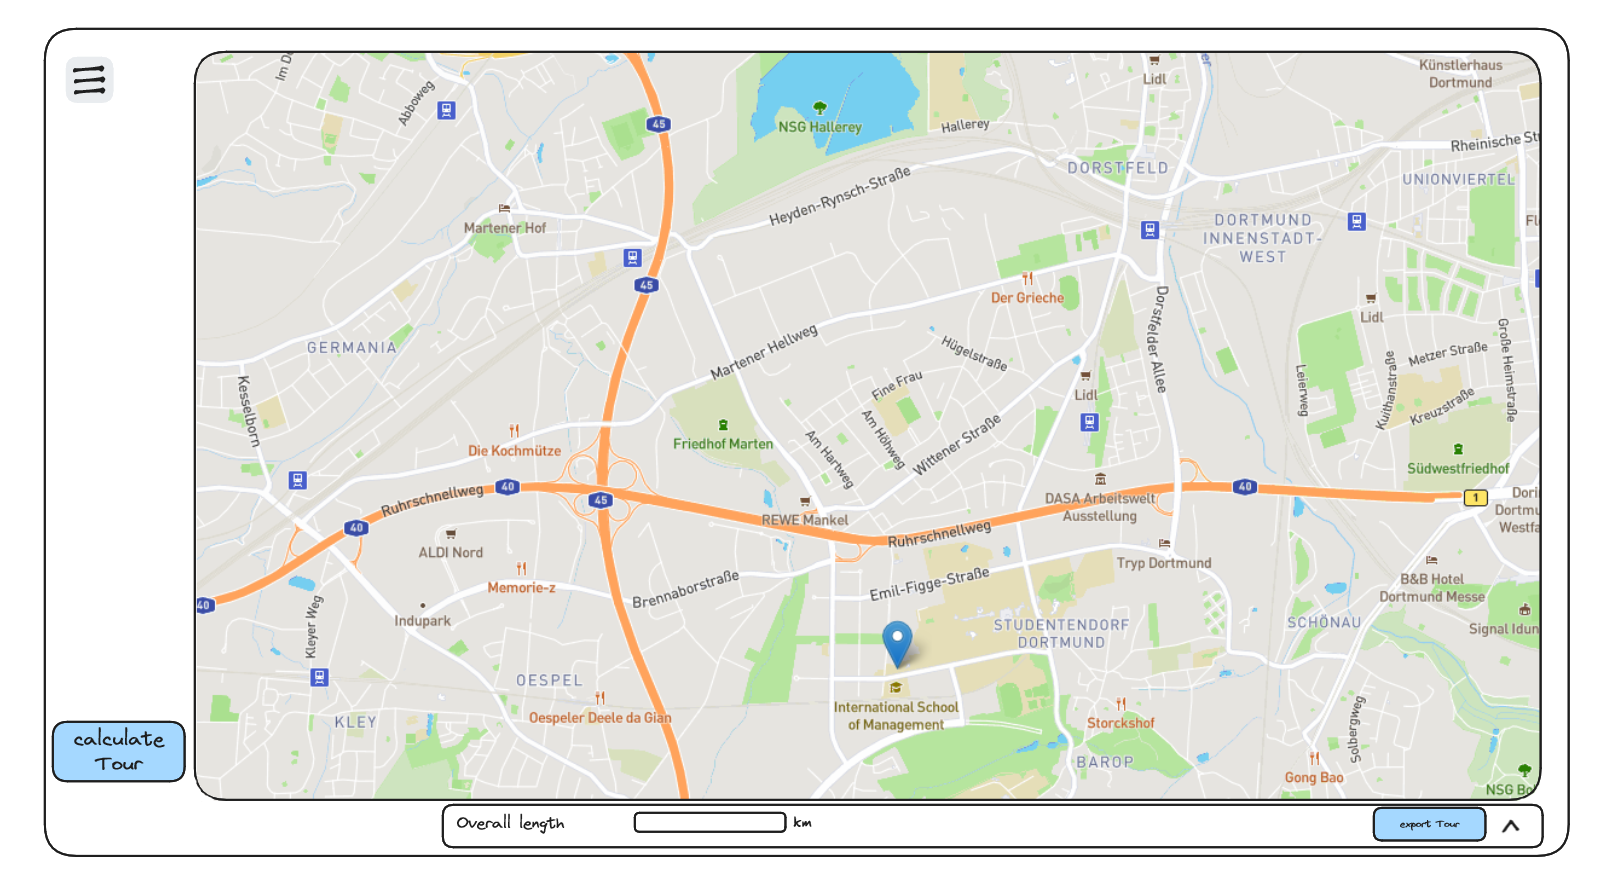
\includegraphics[width=0.9\linewidth]{bilder/Concept burger menu and stats hidden.png}
	\caption{Design concept for the front end view with all menus folded}
	\label{fig:frontendConceptMenusClosed}
\end{figure}


\begin{figure}[H]
	\begin{subfigure}[t]{0.9\linewidth}
		\centering
		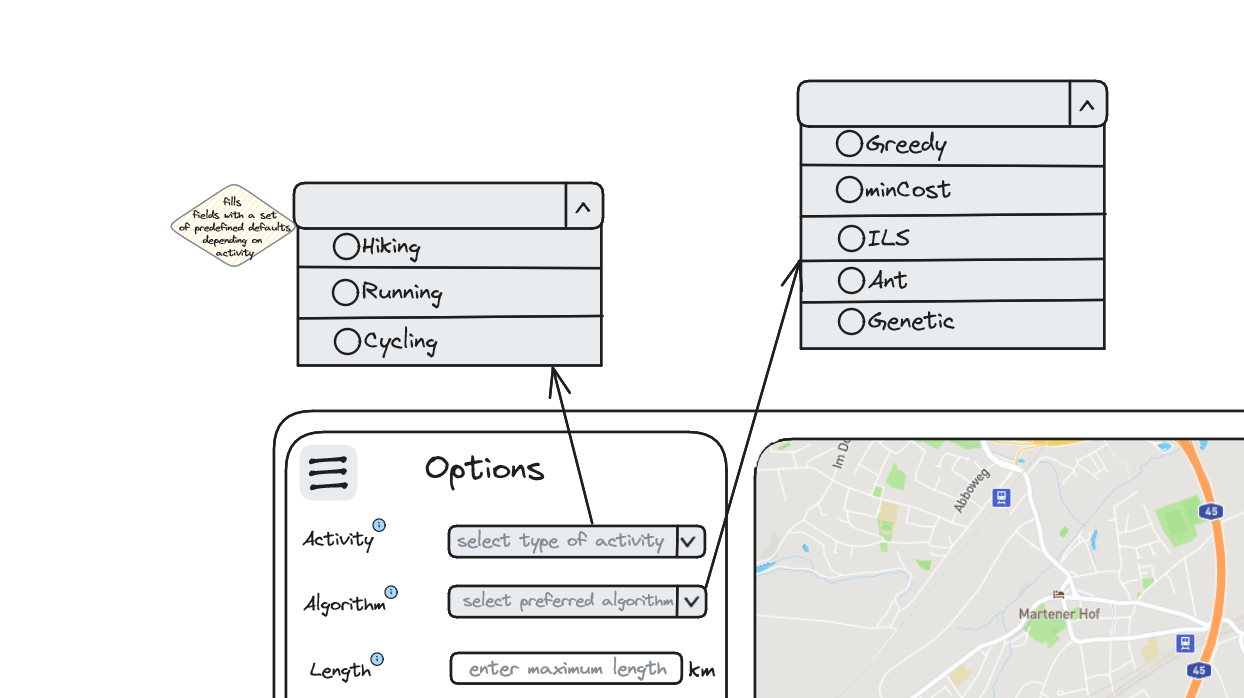
\includegraphics[width=\linewidth]{bilder/Concept closeup activity, algorithm.png}
		\caption{Design concept for the front end view, closeup of activity and algorithm dropdowns}
		\label{fig:frontendConceptCloseupDropdowns}	
	\end{subfigure}
	\hfill
	\begin{subfigure}[t]{0.9\linewidth}
		\centering
		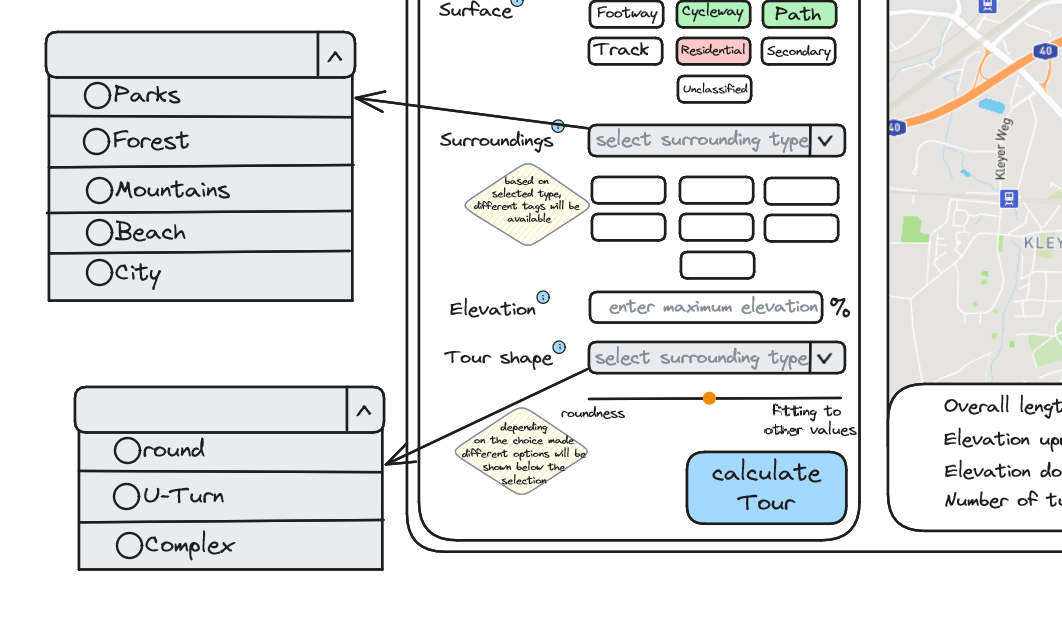
\includegraphics[width=\linewidth]{bilder/Concept closeup surroundings, tour shape.png}
		\caption{Design concept for the front end view, closeup of a surrounding and Tour shape}
		\label{fig:frontendConceptCloseupButtons}		
	\end{subfigure}
	\caption{Closeups of the side menu design concept}
	\label{fig:frontendSideMenuCloseups}
\end{figure}


\begin{figure}[H]
	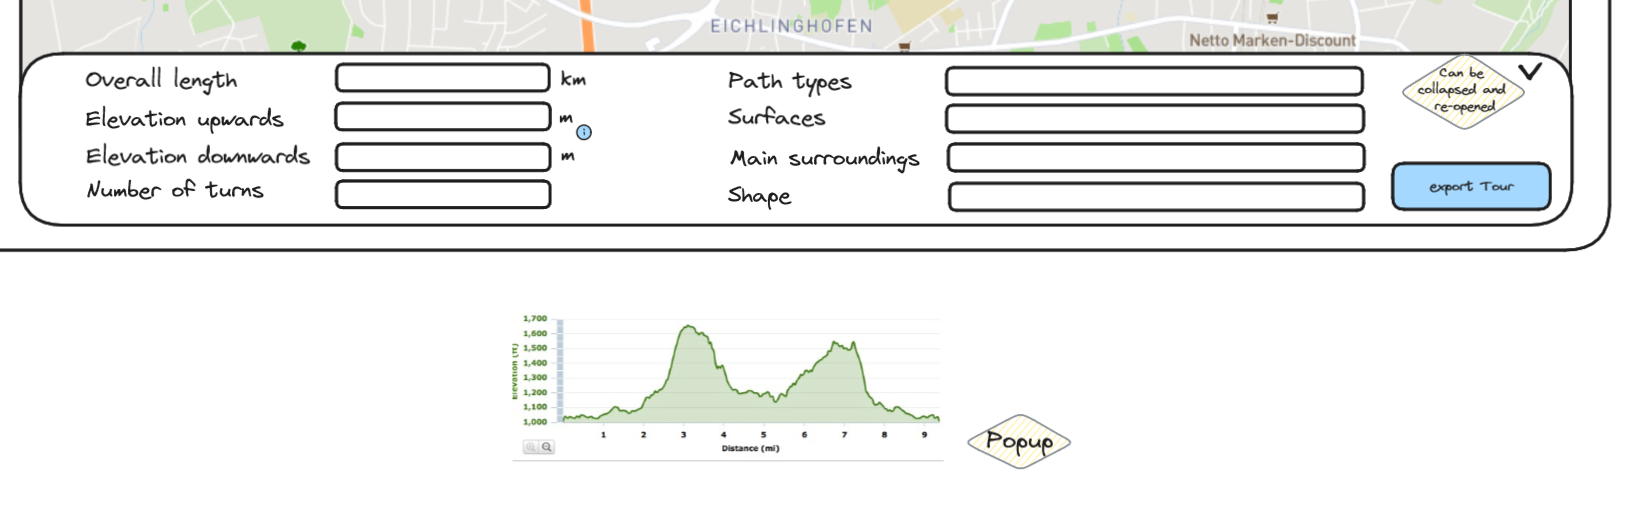
\includegraphics[width=0.9\linewidth]{bilder/Concept closeup tour stats, elevation profile.png}
	\caption{Design concept for the front end view, closeup of the results view}
	\label{fig:frontendConceptResultsCloseup}
\end{figure}

\begin{figure}[H]
	\includegraphics[width=0.9\linewidth]{bilder/actualFrontendSideMenuActivity.png}
	\caption{The options to choose from when the Activity drop down is clicked}
	\label{fig:actualFrontendSideMenuActivity}
\end{figure}


\begin{figure}[H]
	\includegraphics[width=0.9\linewidth]{bilder/actualFrontendSideMenuAlgorithm.png}
	\caption{The options to choose from when the Algorithm drop down is clicked}
	\label{fig:actualFrontendSideMenuAlgorithm}
\end{figure}


\begin{figure}[H]
	\includegraphics[width=0.9\linewidth]{bilder/actualFrontendSideMenuSurroundings.png}
	\caption{The options to choose from when the Surroundings drop down is clicked}
	\label{fig:actualFrontendSideMenuSurroundings}
\end{figure}


\begin{figure}[H]
	\includegraphics[width=0.9\linewidth]{bilder/actualFrontendSideMenuTourShape.png}
	\caption{The options to choose from when the TourShape drop down is clicked}
	\label{fig:actualFrontendSideMenuTourShape}
\end{figure}




\begin{breakablealgorithm}
	\caption{Simulated Annealing}
	\label{alg:SAImplementation}
	\begin{algorithmic}[1]
		\STATE build waypoint list (starting point only)
		\STATE (optional; for weighted selection of points) calculateDistances
		\STATE calculate probability distribution
		\STATE Select init temperature (t)
		\FOR{$i=0$ to numberRepitions}
		\FOR{$i=0$ to numberRuns per temperature}
		\STATE Generate neighborhood roundtrip (j)
		\STATE Calculate difference in quality d = f(j)-f(i)
		\IF {d $\geq$ 0}
		\STATE use neighboring solution as current best i $\gets$ j
		\ELSE 
		\STATE random $\gets$ generate random(0,1)
		\IF {random < exp(d/t)} 
		\STATE use neighboring solution as current best i $\gets$ j
		\ENDIF
		\ENDIF
		\ENDFOR
		\STATE update temperature t $\gets$ T(t)
		\ENDFOR
	\end{algorithmic}
\end{breakablealgorithm}



\begin{breakablealgorithm}
	\caption{Add waypoint}
	\label{alg:SAGenerateNeigborhoodAdd}
	\begin{algorithmic}[1]
		\STATE calculate shortest path between closest waypoint (a) and new point (n)
		\STATE calculate shortest path between new point and closer one of the neighbors of closest waypoint (b)
		\STATE update path from closest waypoint a
		\STATE add new point n into waypoint list
		\STATE update path from new point n to b
		\STATE update full tour to include path part a-n-b
	\end{algorithmic}
\end{breakablealgorithm}

\begin{breakablealgorithm}
	\caption{Move closest waypoint}
	\label{alg:SAGenerateNeigborhoodMove}
	\begin{algorithmic}[1]
		\STATE calculate shortest path between predecessor of closest waypoint (a) and new point (n)
		\STATE calculate shortest path between new point and successor of closest waypoint (b)
		\STATE update path from successor of closest waypoint a
		\STATE update closest waypoint to be the new point n in waypoint list
		\STATE update path from new point n to b
		\STATE update full tour to include path part a-n-b
	\end{algorithmic}
\end{breakablealgorithm}

\begin{breakablealgorithm}
	\caption{Remove closest waypoint}
	\label{alg:SAGenerateNeigborhoodRemove}
	\begin{algorithmic}[1]
		\STATE calculate shortest path between predecessor of closest waypoint (a) and successor of closest waypoint (b)
		\STATE update path from successor of closest waypoint a
		\STATE remove closest waypoint from waypoint list
		\STATE update full tour to only include path part a-b
	\end{algorithmic}
\end{breakablealgorithm}

